% !TeX root = ../../main.tex
% Add the above to each chapter to make compiling the PDF easier in some editors.

\section{Basics of Machine Learning and Deep Learning}\label{ord:ch2:sec1}

In the last decade the development and research interest in the field of \gls{ml} have greatly increased and drawn much attention. 
This section briefly recaptures the fundamental concepts of \gls{ml} and \gls{dl}.
A detailed description of the introduced concepts and terms can be reviewed in \cite{Ger17-HandsOn} or \cite{Goodfellow-et-al-2016}.

%The last decade was revolutionary for the sector of information technology.
%Due to technical advancement, the computational power of processors, especially \gls{gpu} rise significantly.
%Further, the wider creation and use of data introduced the domain of big data, that allows operators to gain more insights and benefits.
%Both of these recent advancements benefited another field of study commonly described as \gls{ai}.
%The term \gls{ai} describes machines that are show characteristics of human intelligence that allow them to handle various tasks.
%But there are several gradations, that hide behind the powerful bus word \gls{ai} and are illustrated in this section.

\subsection{Machine Learning}\label{ord:ch2:sec1:subsec1}

\gls{ml} is the science of creating algorithms, to analyze, detect and learn patterns in various kinds of data without defining explicit decision rules.
These algorithms may achieve human level performance, but mostly they are limited to a single task.
In order to solve another task a \gls{ml} algorithm, has to learn the patterns of the new task from a corresponding dataset $\mathcal{D}$.
As \gls{ml} algorithms aim to model reality, they are also referred to as \gls{ml} model.

% Dataset 
The dataset $\mathcal{D}$ usually is split into a training set $\mathcal{S}$, a test set $\mathcal{S}_2$ and validation set $\mathcal{S}_3$.
These three types of datasets are treated separately, while the \gls{ml} model uses the training set $\mathcal{S}$ to extract the patterns, the test set $\mathcal{S}_2$ and validation set $\mathcal{S}_3$ are only used to evaluate the performance of the model.

% Input x and label y
A dataset $\mathcal{D}$ contains $N$ elements with each element having $M$ features.
An element $\textbf{x}$ can be represented as feature-vector $\textbf{x} = [x_1, \dots ,x_M]$, which the model takes as input.
For the task of supervised learning, the dataset $\mathcal{D}$ consists out of pairs $(\textbf{x}_n, y_n)$. Each input $\textbf{x}_i$ contains a corresponding label $y_i$.
In the scope of classification, this label $y$ is represented by one out of $K$ classes $y \in \lbrace c_1, \dots, c_K \rbrace$.
The classification task is defined as  
\begin{equation}
	f: \mathbb{R}^M \rightarrow \lbrace c_1,\ldots,c_K \rbrace, \quad \textbf{x} \mapsto y
\end{equation}
In order to create a functioning model, the model is trained by adjusting it's inner parameters, referred to as $ \theta $ the weights of the model.
While training a model, the weights are adjusted based on the features are extracted iteratively from the given input $\textbf{x}$.

% Model prediction
The function $f$ describes the model, which computes the estimated output $\hat{y}$ based on the input $\textbf{x}$
\begin{equation}
	\hat y = f(\textbf{x}, \theta)
\end{equation}
with $\hat{y}$ being also referred to as prediction of the model and $ \theta $ as the weights of the model.

% Loss function and Backpropagation
In order to perform a training, the model requires a loss function $L(y,\hat{y})$.
The loss function $L$ calculates the loss of the model based on the difference of the prediction $\hat{y}$ and the true label $y$.
There exist different loss functions to calculate various types of losses.
Depending on the loss the weights of the model are adjusted, to make a better prediction and reduce the error.
Usually, an algorithm called backpropagation \cite{Lin76-Backprob} is used to derive the gradient of the loss with respect to all the weights of the model.
With this, \gls{sgd} can be used to iteratively update the weights and optimize the model.
In the context of \gls{ml} the term \textit{learning} refers to this process.

% Generalization error of a model
The goodness of a model can be defined by the performance on the training set $\mathcal{S}$, test set $\mathcal{S}_2$, and validation set $\mathcal{S}_3$.
The two main causes of failure are underfitted or overfitted models.
An underfitted model is not complex enough to understand the interrelations in the data and, therefore, does not perform well.
Common reasons for underfitted models are missing complexity in the model architecture or too small and not representative datasets.
Overfitted models perform great on the training set $\mathcal{S}$, but poorly on the test set $\mathcal{S}_2$ and validation set $\mathcal{S}_3$.
This happens, when the model does not generalize well enough and instead learns the features of the training set by heart.
To successfully train a model, a tradeoff between overfitting and underfitting must be found.

% Hyperparameter
Further, there exist so-called \textit{hyperparameters}, that are used to adjust the training process or the model architecture.
Important hyperparameters are the learning rate $\lambda$ , the number of training epochs $n_{epochs}$, activation function, and the applied optimizer.


\subsection{Deep Learning}\label{ord:ch2:sec1:subsec2}

For this thesis, it is assumed that the reader is already familiar with the field of \gls{dl} as this subsection only provides a brief introduction. 
If this is not the case, \cite{Goodfellow-et-al-2016} and \cite{Ger17-HandsOn} provide a detailed introduction to this topic.
A \gls{nn} is one of the standard \gls{ml} methods and consists out of multiple neurons.
The architecture principle is characterized by layer-wise order of the neurons.
Similar as for basic \gls{ml} models, a \gls{nn} processes an input $ \textbf{x} $ to create a prediction $ \hat{y} $, which for the task of classification is a class $ c_i $.
If an architecture consists out of multiple layers, the network is also described as \textit{deep}, resulting in the terms \gls{dl} and \gls{dnn}.
The neurons are connected layer by layer, each neuron receives $ n $ inputs $ \left[\textbf{x}_1, \dots \textbf{x}_n \right] $ from the previous layer and passes the output to the next layer.
A neuron sums its input values and applies an activation function to create an output, a frequently used activation function is the \gls{relu} function, an overview is provided in \Cite{SSA20-Activationfunctions}. 

Each connection between neurons is weighted, which determines the relevance of the input $ \textbf{x}_i $ for the individual neuron.
This is done by weights $ \theta $, which are adjusted during the training as the model is in the \textit{learning} process as described previously.

Nowadays, in order to solve various tasks, a variety of different network types exist \eg convolutional, graph or recurrent neural networks.
For the popular task of image processing \glspl{cnn} have proven themselves to be most adequate to classify, localize, or segment objects in images.
The main component of \glspl{cnn} are convolutional layers, that are used to process and extract features from visual input as shown in Figure \ref{fig:ch2:sec1:cnn}.
In these layers a convolution operation is performed on the input by applying $c$ convolution kernels.
The output of a layer is defined as a feature map $F_c$, with also $c$ representing the amount of channels in the feature map.
Further, pooling layers are commonly used, in order to reduce the size of feature maps.
\begin{figure}
	\centering
	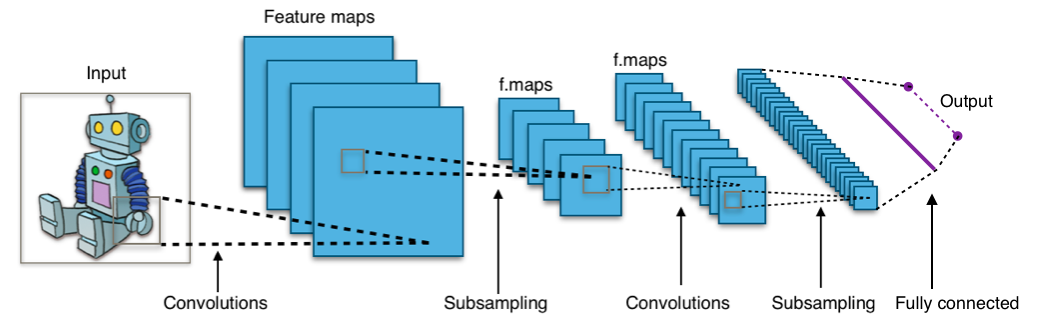
\includegraphics[width=0.8\textwidth]{figures/chap21_cnn.png}
	\caption[Illustration of a CNN]{
		Illustration of a common \gls{cnn} with multiple layers.
		Here the layer-wise architecture is visualized and various layer types are displayed.
		\copyright 2015 CC BY-SA 4.0. Reprinted by permission.\footnotemark 
		
	} \label{fig:ch2:sec1:cnn}
\end{figure}
% CC BY-SA 4.0 - Wikimedia Commons
\footnotetext{Aphex34, 2015, \textit{Typical CNN} \url{https://commons.wikimedia.org/wiki/File:Typical_cnn.png}}

\subsection{Evaluation}\label{ord:ch2:sec1:subsec3}

The performance of a model may be evaluated using various metrics.
In the context of classification, the \textit{true positives} are the number of instances, that are correctly predicted to belong to a certain class $c_i$.
While the \textit{false positives} are the number of instances, that are incorrectly predicted to be positive, but truly are negative.
The contradictory definition applies for the equivalent terms \textit{true negatives} and \textit{false negatives}.

% Accuracy
%\begin{equation}
%	Accuracy = \frac{\textnormal{\textit{true positives}} + \textnormal{\textit{true negatives}}}{\textnormal{\textit{true positives}} + \textnormal{\textit{false positives}} + \textnormal{\textit{true negatives}} + \textnormal{\textit{false negatives}}}
% \end{equation}
The accuracy is one of the most simple metrics and represents the number of correct predictions over the number of all predictions.
To further gain deeper insights on the behavior of models there exist more evaluation metrics as precision and recall \cite{Ger17-HandsOn}.
% precision
%The precision is defined by
%\begin{equation}
%	precision = \frac{\textnormal{\textit{true positives}}}{\textnormal{\textit{true positives}} + \textnormal{\textit{false positives}}}
%\end{equation}
%and represents the accuracy of the positive predictions.
% recall
%The recall is defined by
%\begin{equation}
%	recall = \frac{\textnormal{\textit{true positives}}}{\textnormal{\textit{true positives}} + \textnormal{\textit{false negatives}}}
%\end{equation}
%and is also referred to as \textit{sensitivity} or \textit{true positve rate}.
%The recall describes the ratio of positive instances, that are predicted correctly \cite{Ger17-HandsOn}.

% Further, there exist methods for the evaluation of model as the \textit{F1-Score} or the ROC curve, that are described in \cite{Ger17-HandsOn}.